\chapter{Herramientas de Dibujo 2D}

\begin{figure}[H]
	\centering
	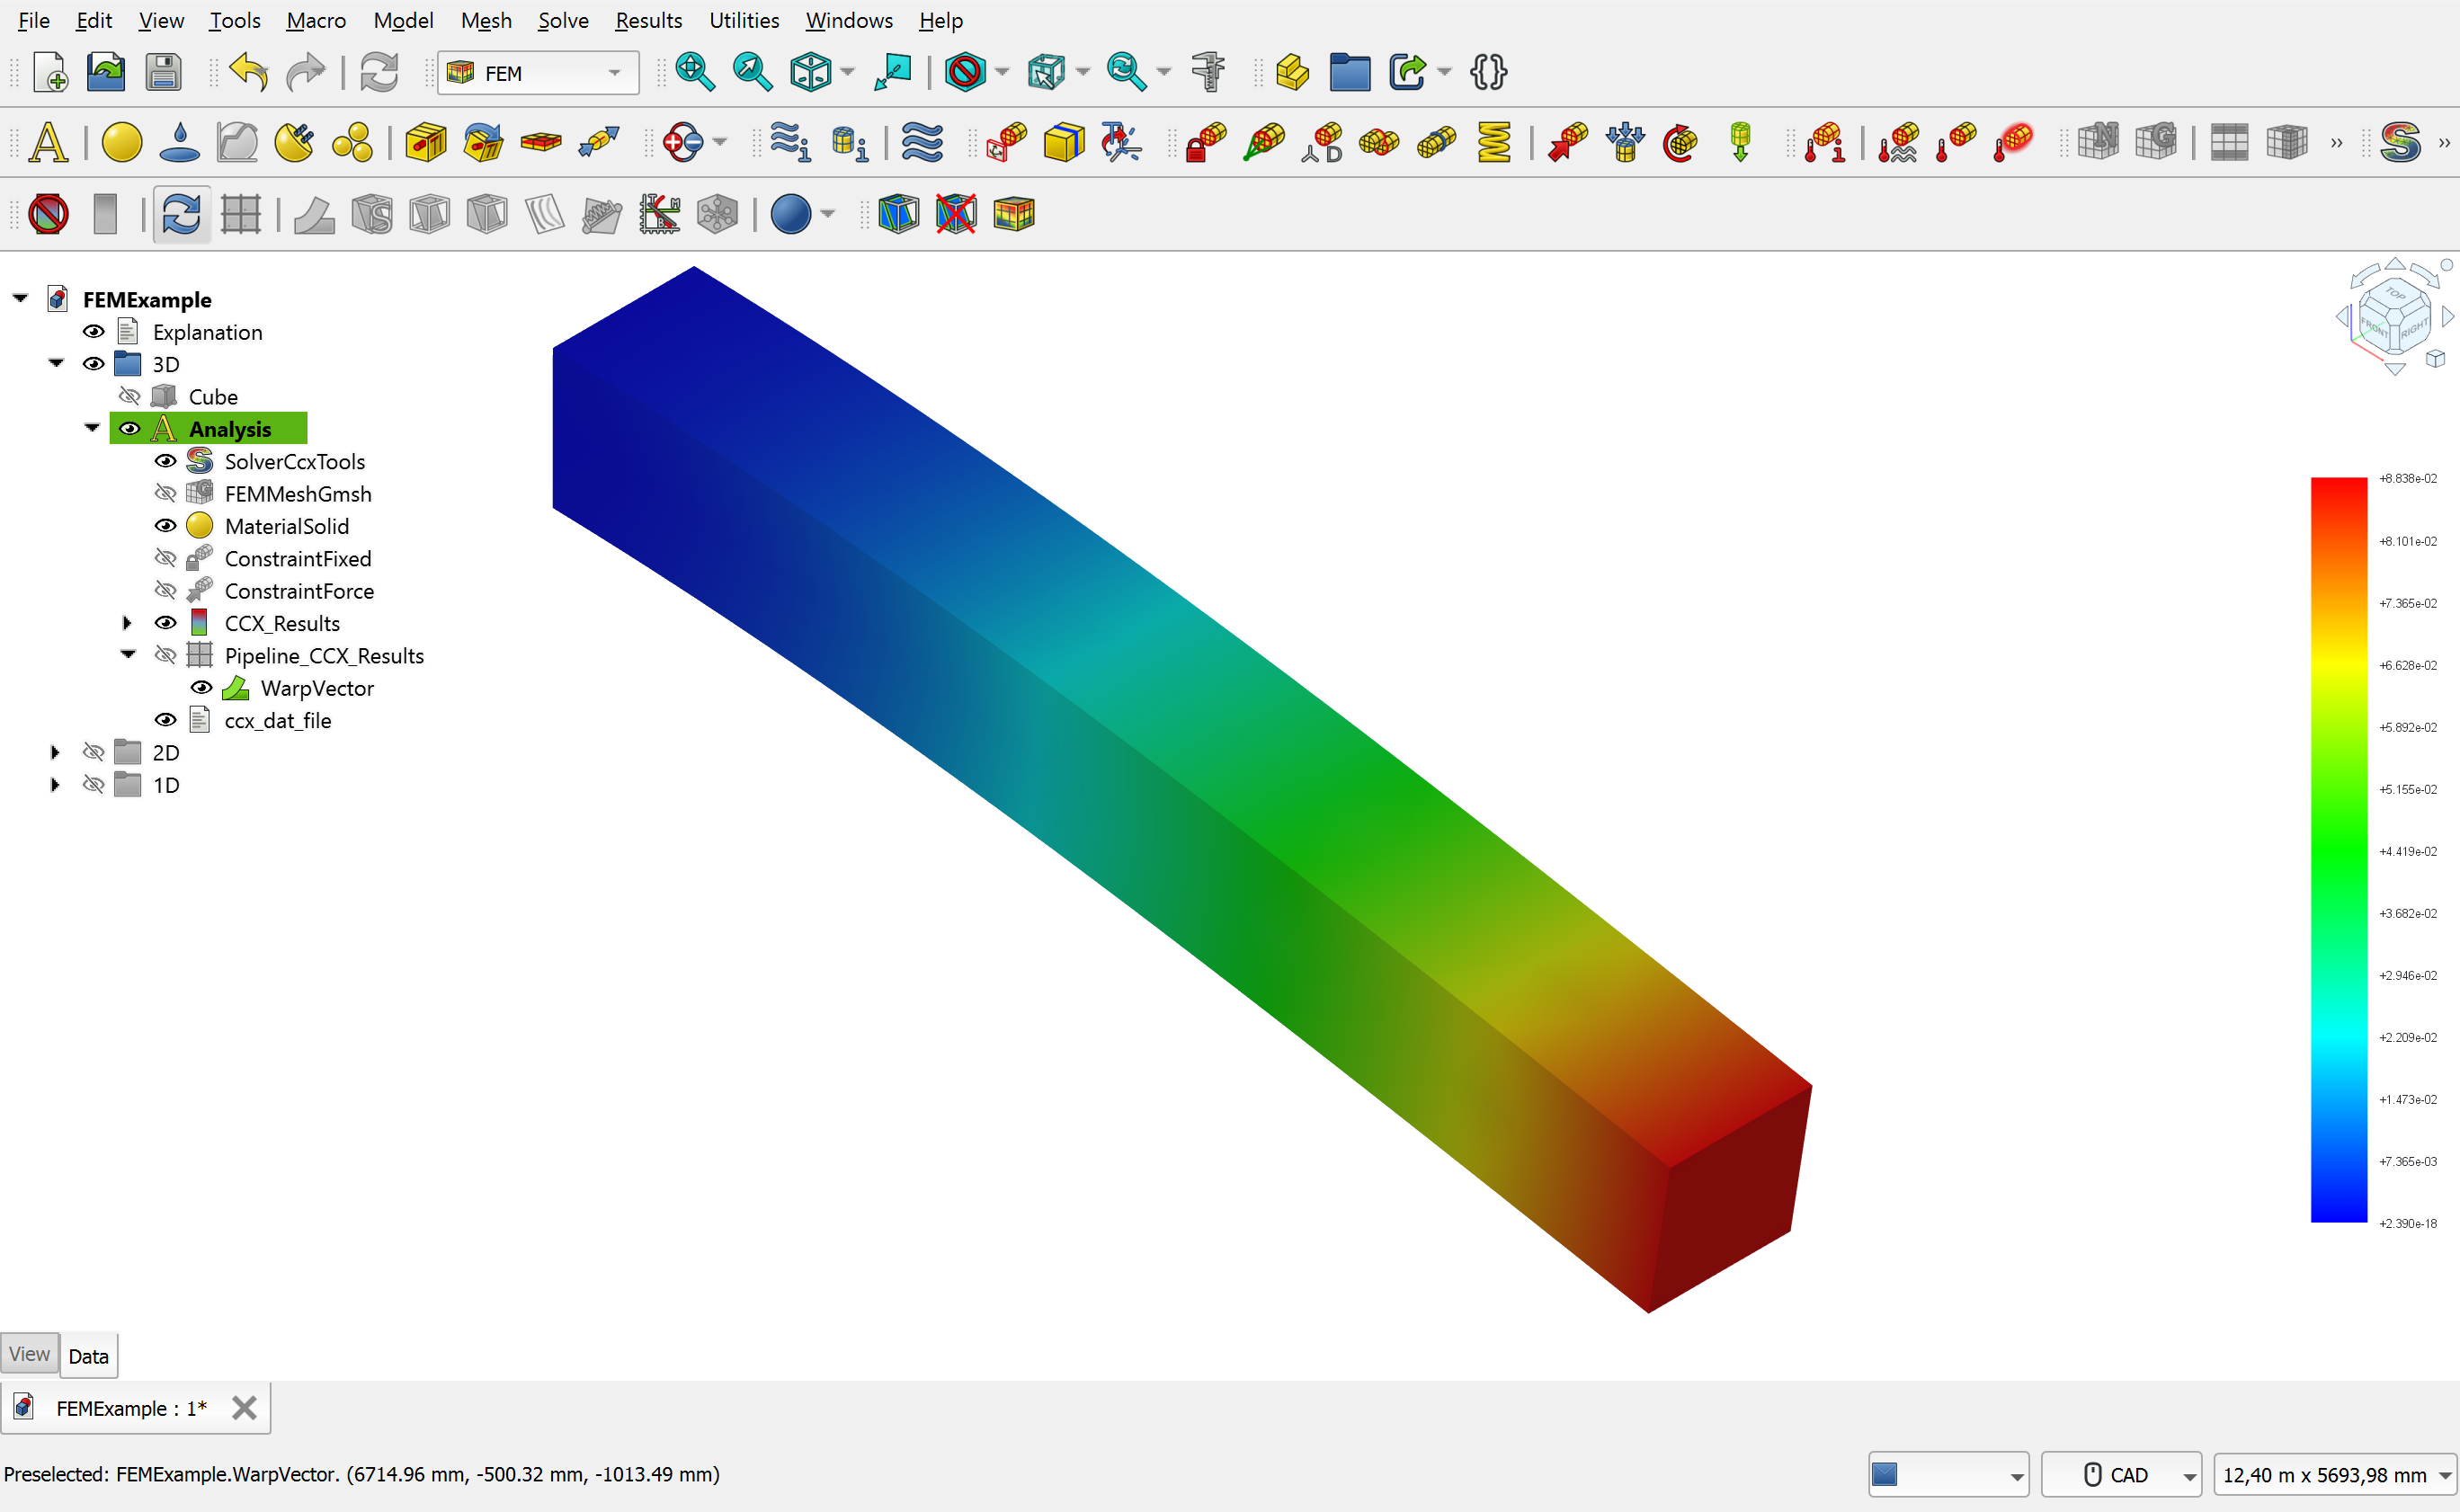
\includegraphics[width=0.8\textwidth]{img/cap3_dibujo2d.png}
	\caption{Área de dibujo 2D con elementos geométricos en FreeCAD}
\end{figure}

Aprende a usar las herramientas de dibujo 2D en FreeCAD.
Crea formas básicas y complejas usando el módulo Sketcher.

%% D. Búsqueda e Inserción de Activos Gráficos
%% Imagen insertada al inicio del capítulo

%% B. Actividades Teóricas
\section{Investigar y responder}
\faPencil

Investiga sobre dibujo 2D en FreeCAD y responde:
\begin{enumerate}
	\item ¿Qué es un boceto o sketch en FreeCAD?
	\item ¿Cuáles son las herramientas básicas de dibujo 2D?
	\item ¿Qué diferencia hay entre líneas, círculos y arcos?
	\item ¿Cómo se crean polígonos regulares e irregulares?
	\item ¿Qué son las polilíneas y cuándo se utilizan?
	\item ¿Cómo importar geometría 2D desde archivos DXF?
	\item ¿Qué herramientas sirven para modificar formas 2D?
	\item ¿Cómo trabajar con capas en dibujo 2D?
\end{enumerate}

%% C. Actividades Prácticas
\section{Resolver los siguientes problemas}
\faWrench

Problemas para aplicar conocimientos:
\begin{enumerate}
	\item Crea un nuevo archivo y activa el módulo Sketcher.
	\item Dibuja un rectángulo de 100x50 mm con
	      dimensiones exactas.
	\item Crea un círculo de radio 25 mm en el centro del
	      plano.
	\item Dibuja un triángulo equilátero de lado 40 mm.
	\item Crea una figura combinando rectángulos y círculos
	      para formar una llave inglesa simple.
	\item Practica el uso de la herramienta de arco con
	      diferentes ángulos.
	\item Dibuja una estrella de cinco puntas usando
	      polilíneas.
	\item Importa un archivo DXF y modifica su geometría.
	\item Crea un plano simple de una pieza mecánica básica.
	\item Organiza tus dibujos en diferentes capas y
	      asigna colores.
\end{enumerate}